\chapterimage{images/future.jpg} % Chapter heading image

\chapter{FutureSystems}
\label{C:futuresystems}
\index{futuresystems}

\FILENAME\

This section gives an overview of the FutureSystems that are available
as part of the DSC infrastructure. We cover the creation of
FutureSystems Account, Uploading SSH Key and how to instantiate and
log into Virtual Machine and accessing Ipython are covered. In the end
we discuss about running Python and Java on Virtual Machine.

\section{FutureSystems evolved from FutureGrid}

In this video we introduce FutureGrid a precurser to FutureSystems.

\video{Systems}{12:12}{FutureGid}{http://youtu.be/RibpNSyd4qg}

At thsi time we are replacing several of the older systems. To use
these new systems you need to ask for access through them via our portal.


\section{Creating Portal Account}

This lesson explains how to create a portal account, which is the first
step in gaining access to FutureSystems.

See Lesson 4 and 7 for SSH key generation on Linux, OSX or Windows.

\video{Python}{11:50}{FutureGrid Introduction}{http://youtu.be/X6zeVEALzTk}

\section{SSH Key Generation using ssh-keygen command}
\label{ssh-key-generation-using-ssh-keygen-command}

SSH keys are used to identify user accounts in most systems including
FutureSystems. This lesson walks you through generating an SSH key via
ssh-keygen command line tool.

\video{Python}{4:06}{ssh-key gen}{http://youtu.be/pQb2VV1zNIc}

\section{Shell Access via SSH}

This lesson explains how to get access FutureSystems resources vis SSH
terminal with your registered SSH key.

\video{Python}{2:34}{Shell Access via SSH}{http://youtu.be/aJDXfvOrzRE}

\section{Advanced SSH}
\index{ssh!Futuresystems}

This lesson shows you how to write SSH `config' file in advanced
settings.

\video{Python}{2:47}{Advanced SSH}{http://youtu.be/eYanElmtqMo}

\section{SSH Key Generation via putty}
\index{putty!Futuresystems}

This lesson is for Windows users. You will learn how to create an SSH
key using PuTTYgen, add the public key to you FutureSystems portal,
and then login using the PuTTY SSH client.

\video{Python}{3:51}{Windows users}{http://youtu.be/irmVJKwWQCU}

\begin{comment}
\section{Creating VMs using Cloudmesh and running IPython}

This lesson explains how to log into FutureSystems and our customized
shell and menu options that will simplify management of the VMs for this
upcoming lessons.

Instruction is at:
\url{http://cloudmesh.github.io/introduction_to_cloud_computing/class/cm-mooc/cm-mooc.html}

\video{Python}{19:28}{Using FS - Creating VM using Cloudmesh and running IPython}{http://youtu.be/nbZbJxheLwc}
\end{comment}

\section{FutureSystems Facilities}\label{S:fs-facilities}

FutureSystems system resources are located at Indiana University
(Bloomington). Resources at Indiana University (Bloomington) include a 

\begin{enumerate}
\item 128-core HP cluster (Bravo), 
\item 92-core cloud cluster (Echo), 
\item 192-core Tesla GPU cluster (Delta),
\item 3456-core Haswell cluster (Juliet), 
\item 126-core NVIDIA K80/Volta GPU cluster (Romeo), 
\item 3264-core Knight's Landing cluster (Tango), 
\item 480-core Platinum cluster (Tempest), 
\item 768-core Platinum cluster (Victor).
\end{enumerate}

Details of the resources are listed in subsequent sections. 

\subsection{Bravo}
\index{FutureSystems!Bravo}

The large-memory HP cluster (Bravo) is a 1.7 Tflop HP Proliant
distributed shared memory cluster with 128 processor cores and 3 TB
total memory capacity. The compute nodes consist of 16 HP DL180
servers, each with two quad-core Intel Xeon E5620 2.4 GHz processors,
192 GB of memory, 12 TB of local attached storage, and a PCIe 4x QDR
InfiniBand adapter for high bandwidth, low-latency MPI
applications. Br avo is currently used as a shared storage cluster and
is not being utilized for compute jobs. Operating System: RedHat Linux
6.9.

\subsection{Delta}
\index{FutureSystems!Delta}

The GPU cluster (Delta) is a SuperMicro distributed shared memory
cluster with 192 CPU cores and 14,336 GPU cores and 3TB total memory
capacity. The compute nodes consist of 16 SuperMicro X8DTG-QF servers,
each with 2 6-core Intel Xeon 5660 2.80 GHz processors, 2 nVIDIA Tesla
C2075 GPUs with 448 cores per GPU, 192GB of memory, 9TB of local
attached storage, and a Mellanox ConnectX-2 VPI dual-port InfiniBand
QDR/10GigE PCIe adapter card. Operating System: RedHat Linux 7.4

\subsection{Echo}
\index{FutureSystems!Echo}

The cloud cluster (Echo) is a SuperMicro distributed shared memory
cluster with 192 CPU cores and 6TB total memory capacity. The compute
nodes consist of 16 SuperMicro X9DRW servers, each node with 2 6-core
Intel(R) Xeon(R) CPU E5-2640 2.50GHz processors; 384GB of memory, 10TB
of local disk storage, a 10GbE Ethernet and a Mellanox ConnectX-3
InfiniBand FDR 56GT/s onboard adapter for high bandwidth, low-latency
MPI applications. Operating System: Ubuntu Linux 16.04

\subsection{Juliet}
\index{FutureSystems!Juliet}

The Haswell cluster (Juliet) is a SuperMicro distributed shared memory
cluster with 3456 CPU cores and 16TB total memory capacity. The
compute nodes consist of SuperMicro X10DRT-HIBF servers, 32 nodes with
2 18-core Intel(R) Xeon(R) CPU E5-2699 v3 2.30GHz processors; 96 nodes
with 2 12-core Intel(R) Xeon(R) CPU E5-2670 v3 2.30GHz processors, all
compute nodes with 128GB of memory, 8TB of local disk storage, 400GB
of NVMe storage, and a Mellanox ConnectX-3 InfiniBand FDR 56GT/s
onboard adapter for high bandwidth, low-latency MPI
applications. Operating System: RedHat Linux 7.4

\subsection{Romeo}
\index{FutureSystems!Romeo}

The K80/Volta GPU cluster (Romeo) is a SuperMicro distributed shared
memory cluster with 126 CPU cores, 161792 CUDA cores, and 768GB total
memory capacity. The compute nodes consist of 4 SuperMicro X10DGQ
servers with 2 12-core Intel(R) Xeon(R) CPU E5-2670 v3 2.30GHz
processors, 4 NVIDIA GK210GL [Tesla K80] GPU Accelerator cards with
4992 CUDA cores, and 2 SuperMicro X10DGO servers with 2 10-core Intel
Xeon E5-2600 v4 2.2GHz processors and 8 NVIDIA V100 (Tesla Volta)
accelerators with 5120 CUDA cores. All nodes with 128GB of memory, 8TB
of local disk storage, 400GB of NVMe storage, and a Mellanox
ConnectX-3 InfiniBand FDR 56GT/s onboard adapter for high bandwidth,
low-latency MPI applications. Operating System: RedHat Linux 7.4

\subsection{Tango}
\index{FutureSystems!Tango}

The Knight's Landing cluster (Tango) is a Penguin Computing
distributed shared memory cluster with 3264 Xeon Phi cores and 12.8TB
total memory capacity. The compute nodes consist of 16 nodes with 1
72-core Intel(R) Xeon Phi(TM) CPU 7290F 1.50GHz processor and 48 nodes
with 1 68-core Intel(R) Xeon Phi(TM) CPU 7250F 1.50GHz processor. All
nodes with 200GB of memory, 3.2TB of local disk storage, 800GB of NVMe
storage, and an Intel OmniPath adapter for high bandwidth, low-latency
MPI applications. Operating System: CentOS release 7.2.1511

\subsection{Tempest}
\index{FutureSystems!Tempest}

The Platinum cluster (Tempest) is a SuperMicro distributed shared
memory cluster with 480 CPU cores and 2.5TB total memory capacity. The
10 compute nodes consist of SuperMicro X11DPT-PS servers with 2
24-core Intel(R) Xeon(R) Platinum 8160 2.10GHz processors, 256GB of
memory, 8TB of local disk storage, 400GB of NVMe storage, and an Intel
OmniPath adapter for high bandwidth, low-latency MPI
applications. Operating System: RedHat Linux 7.4

\subsection{Victor}
\index{FutureSystems!Victor}

The Platinum cluster (Victor) is a SuperMicro distributed shared
memory cluster with 768 CPU cores and 2.5TB total memory capacity. The
16 compute nodes consist of SuperMicro X11DPT-PS servers with 2
24-core Intel(R) Xeon(R) Platinum 8160 2.10GHz processors, 256GB of
memory, 8TB of local disk storage, 400GB of NVMe storage, and a
Mellanox ConnectX-3 InfiniBand FDR 56GT/s adapter for high bandwidth,
low-latency MPI applications. Operating System: RedHat Linux 7.4
(see Figure~\ref{F:victor}).

  \begin{figure}[!htbp]
    \centering
    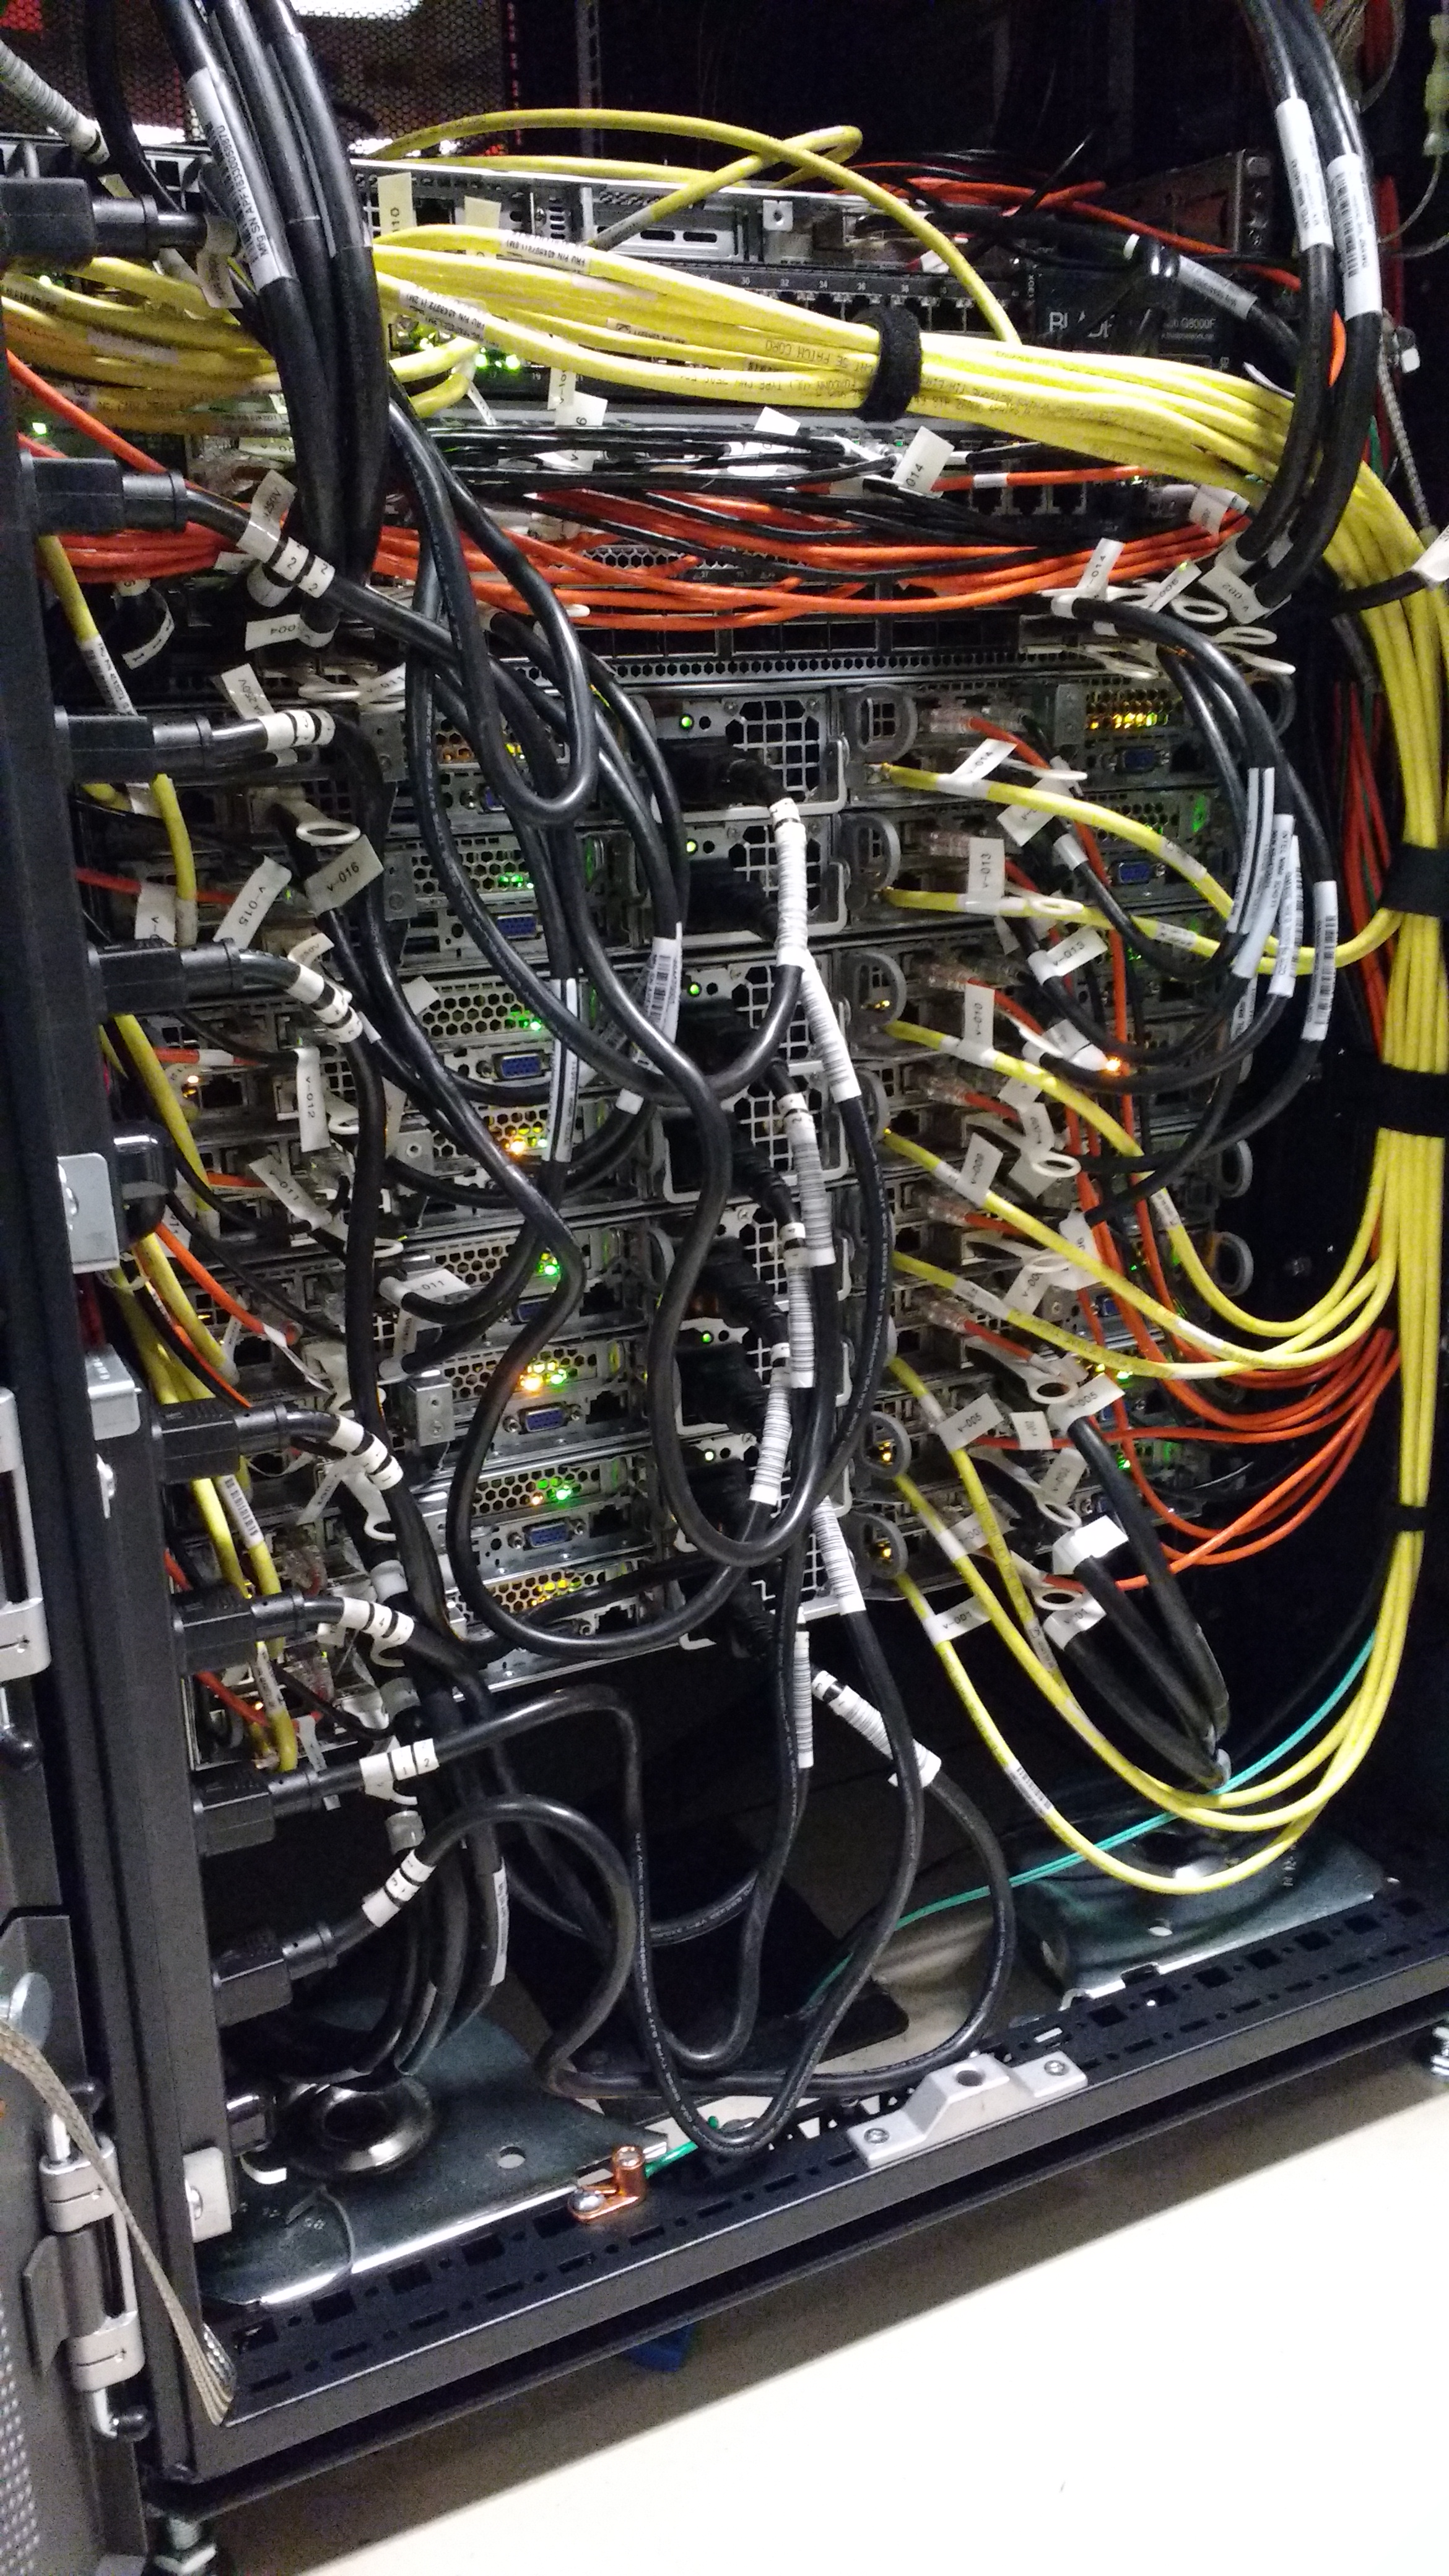
\includegraphics[width=0.9\textwidth]{images/victor.jpg}
    \caption{Cabeling of Victor}\label{F:victor}
  \end{figure}

\subsection{PI Cluster}
\index{FutureSystems!PI Cluster}

The details will be added once we have completed the purchase.
